%\documentstyle[10pt,twoside]{article}
%\documentstyle[twoside]{article}
\documentclass[twoside]{article}
\setlength{\oddsidemargin}{0.25 in}
\setlength{\evensidemargin}{-0.25 in}
\setlength{\topmargin}{-0.6 in}
\setlength{\textwidth}{6.5 in}
\setlength{\textheight}{8.5 in}
\setlength{\headsep}{0.75 in}
\setlength{\parindent}{0 in}
\setlength{\parskip}{0.1 in}

\usepackage{graphicx}
\usepackage{url}

%
% The following commands sets up the lecnum (lecture number)
% counter and make various numbering schemes work relative
% to the lecture number.
%
\newcounter{lecnum}
\renewcommand{\thepage}{\thelecnum-\arabic{page}}
\renewcommand{\thesection}{\thelecnum.\arabic{section}}
\renewcommand{\theequation}{\thelecnum.\arabic{equation}}
\renewcommand{\thefigure}{\thelecnum.\arabic{figure}}
\renewcommand{\thetable}{\thelecnum.\arabic{table}}
\newcommand{\dnl}{\mbox{}\par}

%
% The following macro is used to generate the header.
%
\newcommand{\lecture}[4]{
   \pagestyle{myheadings}
   \thispagestyle{plain}
   \newpage
   \setcounter{lecnum}{#1}
   \setcounter{page}{1}
   \noindent
   \begin{center}
   \framebox{
      \vbox{\vspace{2mm}
    \hbox to 6.28in { {\bf CMPSCI~677~~~Distributed and Operating Systems
                        \hfill Spring 2018} }
       \vspace{4mm}
       \hbox to 6.28in { {\Large \hfill Lecture #1: #2  \hfill} }
       \vspace{2mm}
       \hbox to 6.28in { {\it Lecturer: #3 \hfill Scribe: #4} }
      \vspace{2mm}}
   }
   \end{center}
   \markboth{Lecture #1: #2}{Lecture #1: #2}
   \vspace*{4mm}
}

%
% Convention for citations is authors' initials followed by the year.
% For example, to cite a paper by Leighton and Maggs you would type
% \cite{LM89}, and to cite a paper by Strassen you would type \cite{S69}.
% (To avoid bibliography problems, for now we redefine the \cite command.)
%
\renewcommand{\cite}[1]{[#1]}

% \input{epsf}

%Use this command for a figure; it puts a figure in wherever you want it.
%usage: \fig{NUMBER}{FIGURE-SIZE}{CAPTION}{FILENAME}
\newcommand{\fig}[4]{
            %\vspace{0.2 in}
            \centerline{\includegraphics[scale=#2]{#4}}
            \begin{center}
            Figure \thelecnum.#1:~#3
            \end{center}
    }

% Use these for theorems, lemmas, proofs, etc.
\newtheorem{theorem}{Theorem}[lecnum]
\newtheorem{lemma}[theorem]{Lemma}
\newtheorem{proposition}[theorem]{Proposition}
\newtheorem{claim}[theorem]{Claim}
\newtheorem{corollary}[theorem]{Corollary}
\newtheorem{definition}[theorem]{Definition}
\newenvironment{proof}{{\bf Proof:}}{\hfill\rule{2mm}{2mm}}

% Some useful equation alignment commands, borrowed from TeX
\makeatletter
\def\eqalign#1{\,\vcenter{\openup\jot\m@th
  \ialign{\strut\hfil$\displaystyle{##}$&$\displaystyle{{}##}$\hfil
      \crcr#1\crcr}}\,}
\def\eqalignno#1{\displ@y \tabskip\@centering
  \halign to\displaywidth{\hfil$\displaystyle{##}$\tabskip\z@skip
    &$\displaystyle{{}##}$\hfil\tabskip\@centering
    &\llap{$##$}\tabskip\z@skip\crcr
    #1\crcr}}
\def\leqalignno#1{\displ@y \tabskip\@centering
  \halign to\displaywidth{\hfil$\displaystyle{##}$\tabskip\z@skip
    &$\displaystyle{{}##}$\hfil\tabskip\@centering
    &\kern-\displaywidth\rlap{$##$}\tabskip\displaywidth\crcr
    #1\crcr}}
\makeatother

% **** IF YOU WANT TO DEFINE ADDITIONAL MACROS FOR YOURSELF, PUT THEM HERE:



% Some general latex examples and examples making use of the
% macros follow.

\begin{document}

%FILL IN THE RIGHT INFO.
%\lecture{**LECTURE-NUMBER**}{**DATE**}{**LECTURER**}{**SCRIBE**}
\lecture{5}{February 25}{Prashant Shenoy}{\textbf{Ao Liu}}

\section{Case studies}

\subsection{Volunteer Computing}
Volunteer computing is based on the idea that volunteers donate CPU cycles/storage when it's not in use. A coordinator partitions a large job into small chunks and sends them to the volunteer nodes. Seti@home, BOINC and P2P backups are examples for this paradigm.

\subsection{Condor}
Condor makes use of idle cycles on workstations in a LAN. It can be used to run large batch jobs and long simulations. It has a central job management system, which idle machines contact. They are then assigned jobs. It supports process migration and flexible job scheduling policies.

\subsection{Replicated Web Server}
Here, one of the nodes acts as a load balancing switch and others as replicas. Requests arrive at a queue which acts a load balancer, which employs policies like least loaded or round robin.

\begin{center}
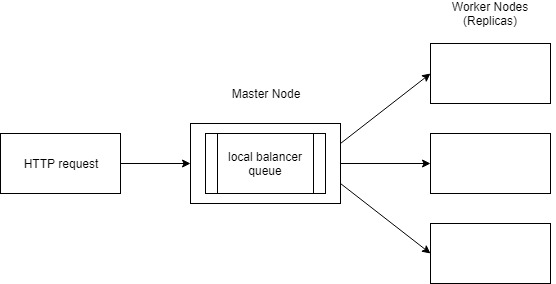
\includegraphics[scale=0.5]{replicated_web_server.jpg}
\end{center}

\section{Virtualization}
Virtualization is the process of providing an interface to
mimic the behavior of another system or components. It can be broadly classified into the following categories:

\subsection{Type of Interfaces}
\begin{itemize}
\item Assembly instructions
\item System calls
\item APIs
\end{itemize}
Depending on what is replaced or mimiced, we obtain different forms of virtualization.

\subsection{Type of Virtualization}

\subsubsection{Emulation}
In emulation, a software simulation of a particular type of hardware is done using another. It can use binary translation to convert instructions on the fly and simulate registers in software. It suffers from the extra overhead of a full implementation.

Examples: Bochs, VirtualPC for Mac, QEMU.

\subsubsection{Full/Native Virtualization}
In native virtualization, one or more OSs and the applications they contain are run on top of virtual hardware. Here, the underlying hardware and virtual hardware are of the same type, but the VM simulates “enough” hardware to allow the OSs to be run in isolation.

Examples: IBM VM family, VMWare Workstation, Parallels, VirtualBox.

\subsubsection{Para-virtualization}
Here, the VM does not simulate hardware. The kernel of the guest OS is modified so that it uses special APIs to call the hypervisor instead of directly accessing the hardware.

Examples: Xen, VMWare ESX Server.

\subsubsection{OS-level Virtualization}

Here the OS allows multiple secure virtual environments to be run. Each application sees an isolated OS. It also serves the use case of backward compatibility.

Examples: Solaris Containers, BSD Jails, Linux Vserver, Linux containers, Docker.

\subsubsection{Application level virtualization}
Here, the application is given its own copy of components that are not shared like global objects, registry files etc.

Example: JVM, Rosetta on Mac (also emulation), WINE.

\subsection{Type of Hypervisors}
Hypervisor/VMM is the virtualization layer, which makes resource management, isolation and scheduling. There are 2 types of hypervisors that act like real hardware. Type 1 hypervisor runs on "bare metal", whereas type 2 hypervisor runs on a host OS and the guest OS runs inside the hypervisor.

\subsection{How Virtualization Works?}
CPU supports kernel (ring 0) and user (ring 3) modes. There is a set of instructions (such as I/O, change MMU settings etc.) that can only be executed in kernel mode. Such instructions are called \textit{sensitive instructions}. Privileged instructions cause a trap when executed in kernel mode. As a result, type 1 virtualization is feasible if sensitive instruction is subset of privileged instructions. Recent Intel/AMD CPUs have hardware support, named Intel VT and AMD SVM. The idea is to create containers where a VM and guest can run and that hypervisor uses hardware bitmap to specify which instruction should trap, so that sensitive instruction in guest traps to hypervisor.

\subsection{Type 1 Hypervisor}
In this type, unmodified OS is running in user mode (or ring 1), but it thinks it's running in kernel mode (\textit{virtual kernel mode}). The guest OS traps on privileged instructions and uses VT to trap sensitive instructions. Under this mode, hypervisor is the "real kernel". Upon trap, it executes privileged operations or emulates what the hardware would do.

\subsection{Type 2 Hypervisor}
Type 2 works without VT support and sensitive instructions are replaced by procedures that emulate them. For example, VMWare, upon loading program, scans code for basic blocks and replaces sensitive instructions by VMWare procedure using binary translation.

\subsection{Para-virtualization}
Both type 1 and 2 hypervisors work on unmodified OS. In contrast, para-virtualization modifies OS kernel to replace all sensitive instructions with hypercalls. Thus, OS behaves like a user program making system calls and hypervisor executes the privileged operation invoked by hypercall.
\end{document}
